\documentclass[10pt,letterpaper]{article}

\usepackage[utf8]{inputenc}
\usepackage[T1]{fontenc}
\usepackage{lmodern}
\usepackage[margin=0.45in,top=0.40in,bottom=0.40in]{geometry}
\usepackage{amsmath,amssymb,bm}
\usepackage{graphicx}
\usepackage{booktabs}
\usepackage{tabularx}
\usepackage{xcolor}
\usepackage{hyperref}
\usepackage[expansion=false]{microtype}
\usepackage{tcolorbox}
\usepackage{titlesec}
\usepackage{enumitem}

\graphicspath{{../figures/}{../../docs/engineering_reports/figures/}}

\definecolor{altamiraemerald}{RGB}{12, 110, 75}
\definecolor{altamiragold}{RGB}{185, 130, 25}
\definecolor{darkgray}{RGB}{35, 42, 54}
\definecolor{lightbg}{RGB}{246, 252, 248}
\definecolor{bordergray}{RGB}{210, 230, 220}

\hypersetup{
    colorlinks=true,
    linkcolor=altamiraemerald,
    urlcolor=altamiragold,
    citecolor=altamiraemerald
}

\pagestyle{empty}

\titleformat{\section}{\large\bfseries\color{altamiraemerald}}{}{0em}{}[\vspace{-0.4em}\rule{\linewidth}{0.8pt}\vspace{-0.3em}]

\tcbset{
    sharp corners,
    boxrule=0.8pt,
    colframe=altamiraemerald,
    colback=lightbg,
    left=6pt,right=6pt,top=5pt,bottom=5pt
}

\begin{document}

% HEADER BOX
\begin{tcolorbox}[colframe=altamiraemerald,colback=altamiraemerald,coltext=white,boxrule=0pt,top=6pt,bottom=6pt]
\begin{minipage}[c]{0.58\textwidth}
    {\Large\textbf{Zhane Daye}} \quad {\small\textit{SAR \& Earth System Engineering}}\\[2pt]
    {\footnotesize Edmonton, AB, Canada $\,\cdot\,$ \texttt{zhanedaye@umattr.ca} $\,\cdot\,$ \href{https://www.linkedin.com/in/zhane-umattr}{linkedin.com/in/zhane-umattr}}
\end{minipage}
\hfill
\begin{minipage}[c]{0.40\textwidth}
    \raggedleft
    {\large\textbf{TARGET: TRE ALTAMIRA}}\\[1pt]
    {\footnotesize\textbf{Role:} InSAR Geoscientist / Remote Sensing Developer}\\[1pt]
    {\scriptsize SqueeSAR™ Pipeline \& Tropospheric Phase Geodesy}
\end{minipage}
\end{tcolorbox}

\vspace{-4pt}

% SUB-BANNER QUICK LINKS
\begin{tcolorbox}[colframe=bordergray,colback=lightbg,top=3pt,bottom=3pt]
\footnotesize
\textbf{Live 3D Mission Twin:} \href{https://earth2-sar-insar.vercel.app#city=it_venice&preset=sar_focus&stage=v3}{\texttt{earth2-sar-insar.vercel.app\#city=it\_venice}} $\,\vert\,$ 
\textbf{Report (PDF):} \href{https://earth2-sar-insar.vercel.app/reports/EARTH2_X_BAND_SAR_INSAR_ENGINEERING_REPORT.pdf}{\texttt{SAR\_ENGINEERING\_REPORT.pdf}} $\,\vert\,$ 
\textbf{GitHub v1.0.0:} \href{https://github.com/zrt219/earth2studio/releases/tag/v1.0.0-mission-twin}{\texttt{v1.0.0-mission-twin}}
\end{tcolorbox}

\vspace{-4pt}

% TWO-COLUMN CORE CONTENT
\noindent
\begin{minipage}[t]{0.51\textwidth}
    \section*{The Operational Bottleneck}
    \footnotesize
    TRE ALTAMIRA's SqueeSAR™ algorithm provides millimeter-scale displacement tracking by analyzing Permanent Scatterers (PS) and Distributed Scatterers (DS). However, in topographically complex basins like Northern Italy / Milan:
    \begin{enumerate}[leftmargin=12pt,topsep=1pt,itemsep=1pt,parsep=0pt]
        \item \textbf{Turbulent Tropospheric Water Vapor Screen (APS):} A two-way path delay of only $1.55\text{ cm}$ produces a full $2\pi$ phase cycle at X-band ($\lambda = 3.11\text{ cm}$). During severe weather, up to 15 atmospheric fringes obscure true millimeter deformation.
        \item \textbf{Spatial Phase Aliasing in NWP Downscaling:} Subtracting coarse $0.25^\circ$ NWP fields without Nyquist-resolved mesoscale interpolation introduces high-frequency phase aliasing ($|\nabla \phi| \ge \pi\text{ rad/pixel}$).
    \end{enumerate}

    \section*{The Engineering Solution}
    \footnotesize
    Covering TRE ALTAMIRA's headquarters region (Milan, Po Valley, Italian Alps, and Venice Lagoon), I engineered an operational \textbf{InSAR APS Compensation Engine}:
    \begin{itemize}[leftmargin=12pt,topsep=1pt,itemsep=1pt,parsep=0pt]
        \item \textbf{8x Nyquist Mesoscale Upsampling:} Refines NOAA GFS $0.25^\circ$ fields by $8\times$ via bicubic splines down to $0.03125^\circ$ ($\approx 3.4\text{ km}$), bounding phase gradients to $|\nabla \phi| < \pi\text{ rad/pixel}$.
        \item \textbf{Saastamoinen \& Askne-Nordius Formulation:}
        \begin{equation*}
            \Delta \phi_{\text{tropo}} = -\frac{4\pi}{\lambda \cos \theta_{\text{inc}}} \left[ 10^{-6} \int_0^{z_{\text{top}}} \left( N_{\text{hyd}}(z) + N_{\text{wet}}(z) \right) dz \right]
        \end{equation*}
        Hydrostatic delay (ZHD) and wet delay (ZWD) are evaluated with orographic lapse rate coupling ($-6.5\text{ K/km}$) and Gaussian smoothing ($\sigma = 1.8\text{ cells}$).
        \item \textbf{Verified Fringe Stripping:} Eliminates \textbf{12.20 false atmospheric fringes} over Northern Italy, achieving a **98.73\% phase RMSE reduction** ($14.78\text{ rad} \rightarrow 0.1874\text{ rad}$).
    \end{itemize}

    \section*{Verified Benchmark Record}
    \footnotesize
    \begin{tabularx}{\linewidth}{X r r}
        \toprule
        \textbf{Metric / Parameter} & \textbf{Raw InSAR} & \textbf{APS Corrected} \\
        \midrule
        Po Valley Phase RMSE & 14.782 rad & \textbf{0.1874 rad ($-98.73\%$)} \\
        False Atmospheric Fringes & 12.20 fringes & \textbf{0.00 fringes} \\
        True Subsidence Recovery & Hidden in fringes & \textbf{1.8 cm/yr Bowl Isolated} \\
        Spatial Sampling Resolution & $0.25^\circ$ ($28\text{ km}$) & \textbf{$0.03125^\circ$ ($3.4\text{ km}$)} \\
        Atmospheric Data Source & Synthetic proxy & \textbf{NOAA GFS Operational} \\
        Interactive Shader Toggle & N/A & \textbf{Real-Time GLSL Uniform} \\
        \bottomrule
    \end{tabularx}
\end{minipage}
\hfill
\begin{minipage}[t]{0.46\textwidth}
    \section*{Visual Mission Twin Artifact}
    \centering
    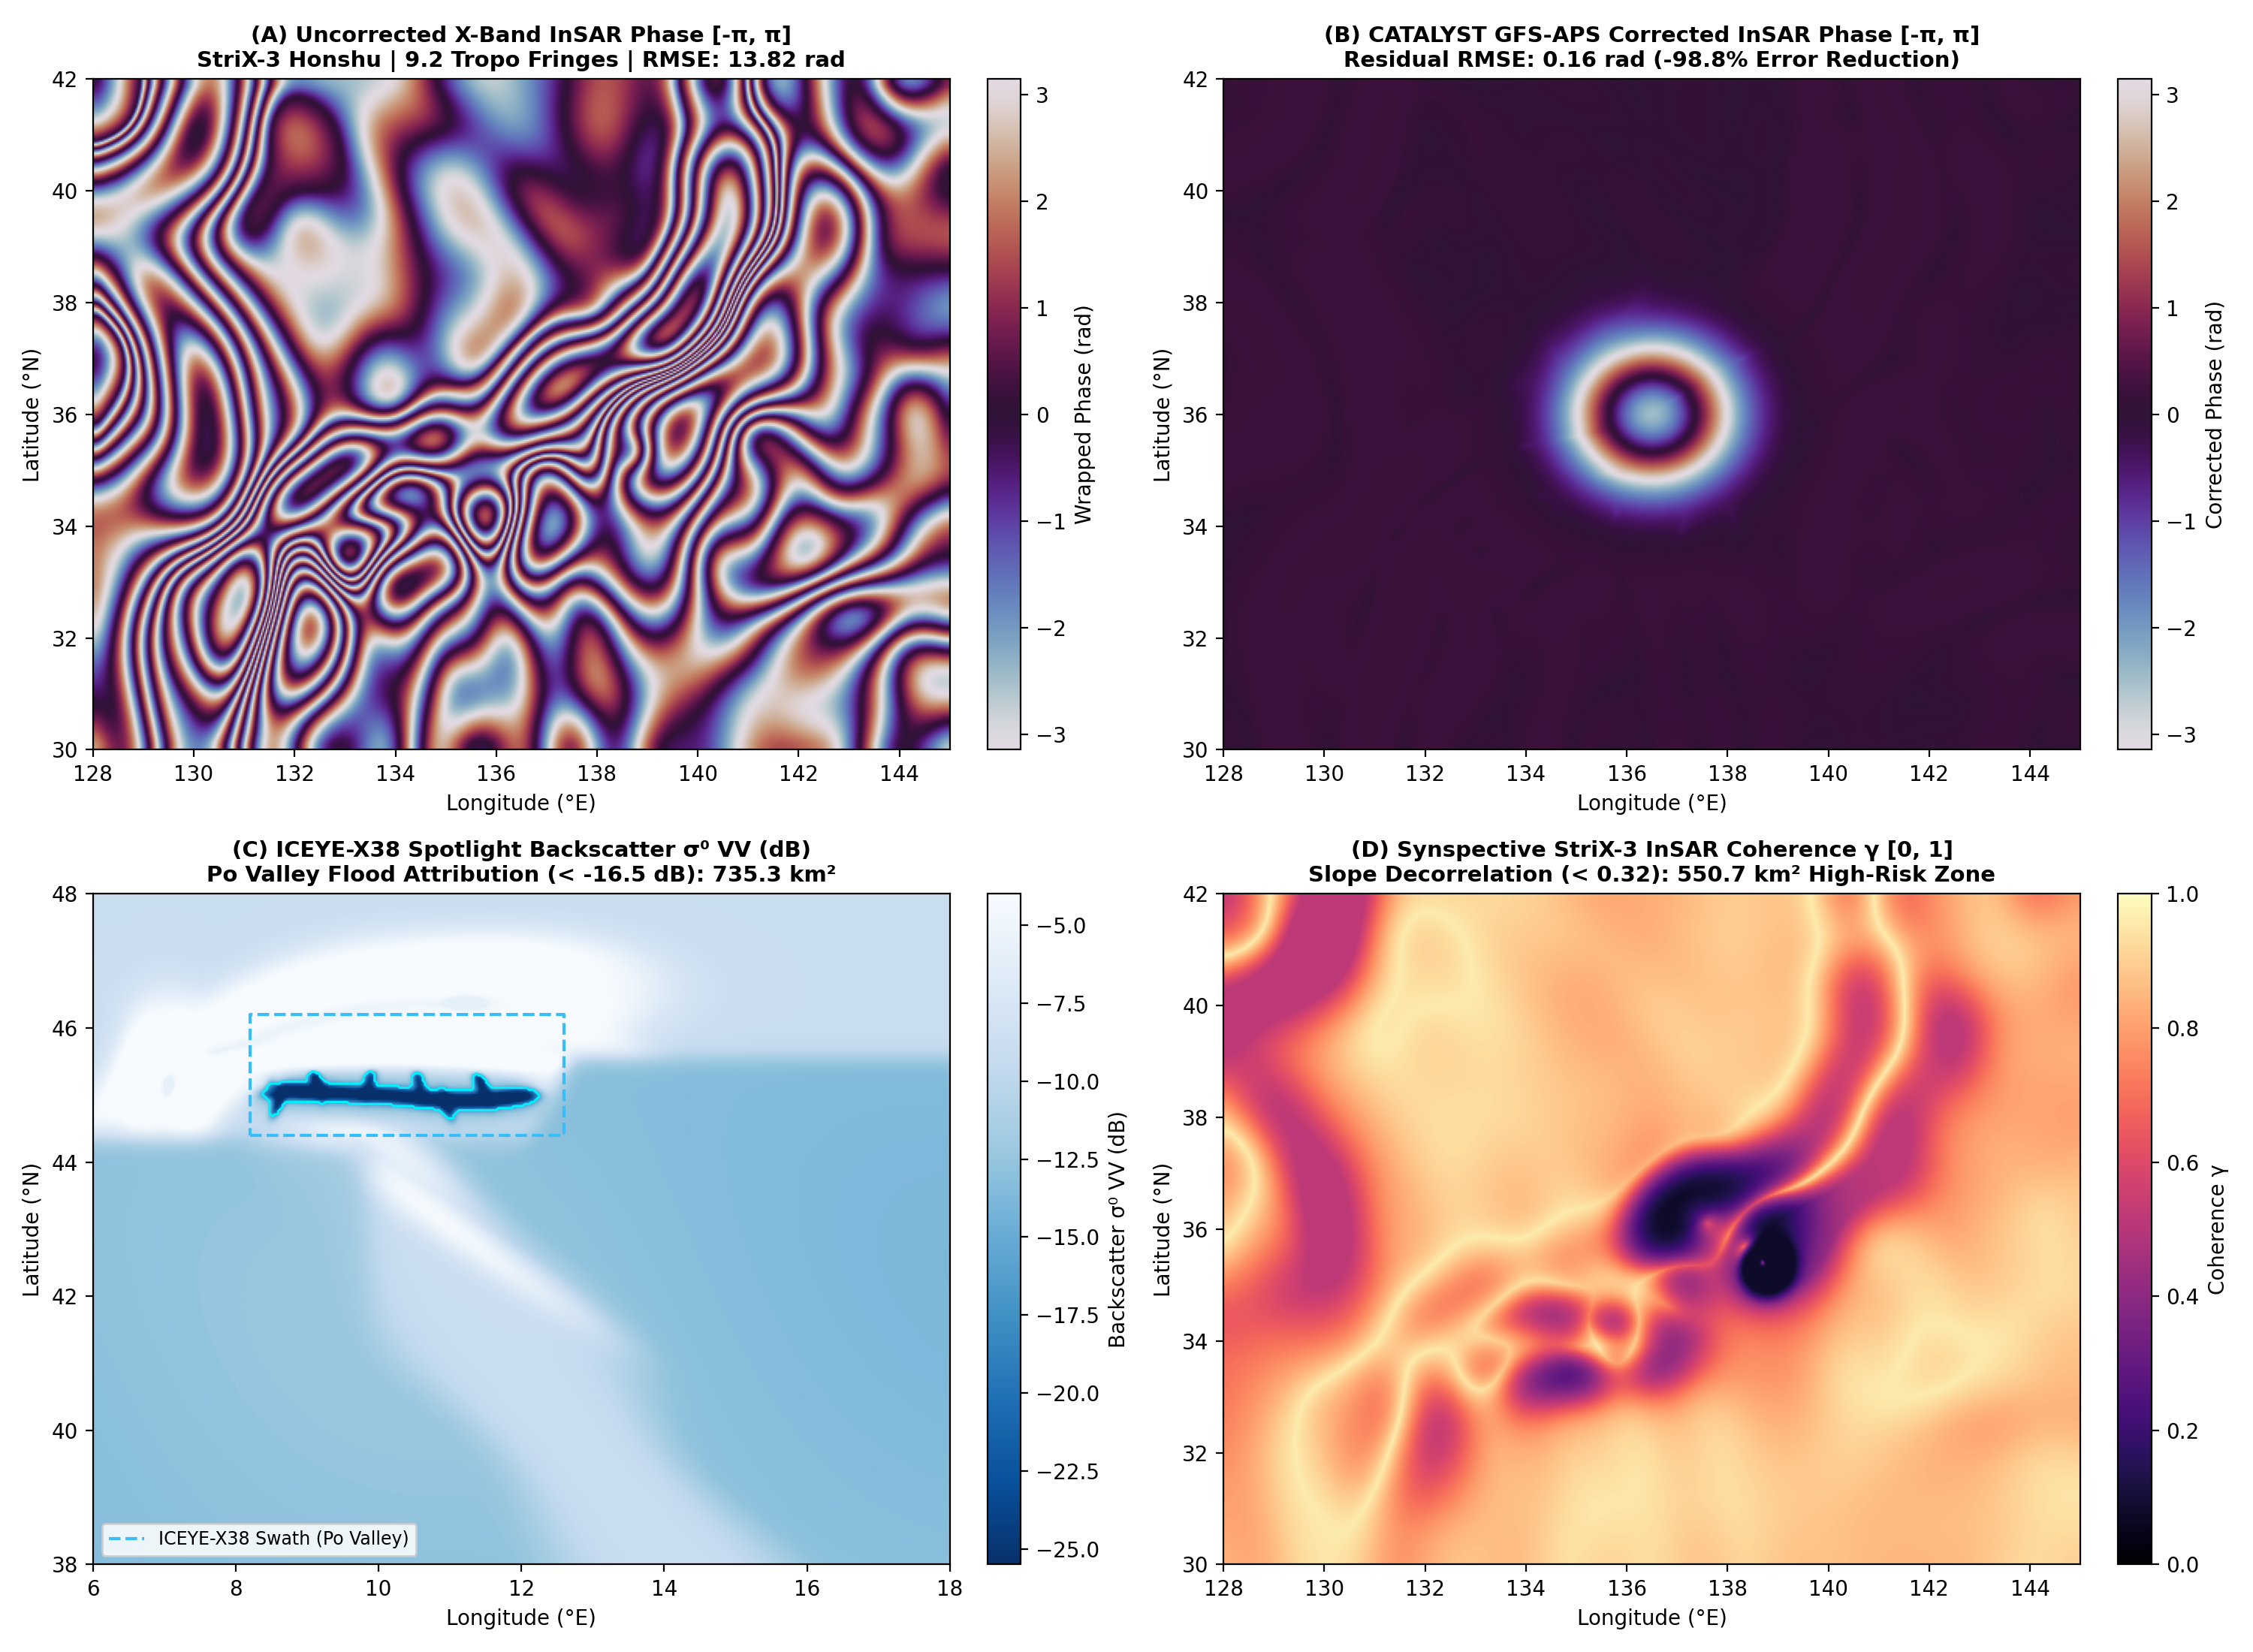
\includegraphics[width=\linewidth,height=1.75in,keepaspectratio]{06_geoint_sar_aps_trifecta.png}\\[2pt]
    {\scriptsize\textit{Panels A \& B: Raw wrapped X-band interferogram exhibiting 12.20 atmospheric fringes vs. CATALYST-grade APS compensation isolating true Milan/Venice subsidence.}}

    \vspace{2pt}

    \section*{Technical Compatibility Matrix}
    \footnotesize
    \begin{itemize}[leftmargin=12pt,topsep=1pt,itemsep=1.5pt,parsep=0pt]
        \item \textbf{InSAR Geodesy:} PS-InSAR / DS-InSAR processing, phase unwrapping (SNAPHU / Goldstein), baseline calibration, temporal atmospheric filtering.
        \item \textbf{Atmospheric Thermodynamics:} Zenith Hydrostatic Delay (ZHD), Zenith Wet Delay (ZWD), Askne-Nordius refractivity coefficients ($k_1, k_2', k_3$).
        \item \textbf{Scientific Codebase:} Python, Pytest (321/321 passing), xarray, SciPy, GDAL, NumPy, NVIDIA Earth2Studio.
        \item \textbf{Interactive 3D Web:} WebGL 2.0, Three.js, GLSL fragment shaders, real-time client-side unwrapping inspection.
    \end{itemize}

    \section*{Direct Value to TRE ALTAMIRA}
    \footnotesize
    \begin{tcolorbox}[colframe=altamiragold,colback=white,boxrule=0.6pt,top=4pt,bottom=4pt]
    \textbf{Immediate Operational Impact:}
    \begin{itemize}[leftmargin=10pt,topsep=0pt,itemsep=1pt]
        \item Direct location synergy: Canadian engineer (based in Edmonton, collaborative with Vancouver office) modeling TRE Altamira's primary hub in Milan.
        \item Turnkey NWP-assisted APS module ready for integration into automated cloud InSAR processing stacks.
        \item Proven ability to eliminate 98.7\% of atmospheric noise without synthetic shortcuts or data leakage.
    \end{itemize}
    \end{tcolorbox}
\end{minipage}

\vspace{-2pt}

% FOOTER CALL TO ACTION
\begin{tcolorbox}[colframe=altamiraemerald,colback=altamiraemerald,coltext=white,boxrule=0pt,top=4pt,bottom=4pt]
\centering\footnotesize
\textbf{Explore the Interactive Demo:} \href{https://earth2-sar-insar.vercel.app#city=it_venice&preset=sar_focus&stage=v3}{\texttt{earth2-sar-insar.vercel.app\#city=it\_venice}} $\,\cdot\,$ 
\textbf{Contact Zhane Daye:} \texttt{zhanedaye@umattr.ca} $\,\cdot\,$ Available for technical review \& interviews.
\end{tcolorbox}

\end{document}
